\documentclass{sigchi}

% Use this section to set the ACM copyright statement (e.g. for
% preprints).  Consult the conference website for the camera-ready
% copyright statement.

% Copyright
%\CopyrightYear{2020}
%\setcopyright{acmcopyright}
%\setcopyright{acmlicensed}
%\setcopyright{rightsretained}
%\setcopyright{usgov}
%\setcopyright{usgovmixed}
%\setcopyright{cagov}
%\setcopyright{cagovmixed}
% DOI
%\doi{https://doi.org/10.1145/3313831.XXXXXXX}
% ISBN
% \isbn{978-1-4503-6708-0/20/04}
%Conference
\conferenceinfo{CHI'20,}{April  25--30, 2020, Honolulu, HI, USA}
%Price

% Use this command to override the default ACM copyright statement
% (e.g. for preprints).  Consult the conference website for the
% camera-ready copyright statement.

%% HOW TO OVERRIDE THE DEFAULT COPYRIGHT STRIP --
%% Please note you need to make sure the copy for your specific
%% license is used here!
% \toappear{
% Permission to make digital or hard copies of all or part of this work
% for personal or classroom use is granted without fee provided that
% copies are not made or distributed for profit or commercial advantage
% and that copies bear this notice and the full citation on the first
% page. Copyrights for components of this work owned by others than ACM
% must be honored. Abstracting with credit is permitted. To copy
% otherwise, or republish, to post on servers or to redistribute to
% lists, requires prior specific permission and/or a fee. Request
% permissions from \href{mailto:Permissions@acm.org}{Permissions@acm.org}. \\
% \emph{CHI '16},  May 07--12, 2016, San Jose, CA, USA \\
% ACM xxx-x-xxxx-xxxx-x/xx/xx\ldots \$15.00 \\
% DOI: \url{http://dx.doi.org/xx.xxxx/xxxxxxx.xxxxxxx}
% }

% Arabic page numbers for submission.  Remove this line to eliminate
% page numbers for the camera ready copy
% \pagenumbering{arabic}

% Load basic packages
\usepackage{balance}       % to better equalize the last page
\usepackage{graphics}      % for EPS, load graphicx instead 
\usepackage[T1]{fontenc}   % for umlauts and other diaeresis
\usepackage{txfonts}
\usepackage{mathptmx}
\usepackage[pdflang={en-US},pdftex]{hyperref}
\usepackage{color}
\usepackage{booktabs}
\usepackage{textcomp}


% Some optional stuff you might like/need.
\usepackage{microtype}        % Improved Tracking and Kerning
% \usepackage[all]{hypcap}    % Fixes bug in hyperref caption linking
\usepackage{ccicons}          % Cite your images correctly!
% \usepackage[utf8]{inputenc} % for a UTF8 editor only

% If you want to use todo notes, marginpars etc. during creation of
% your draft document, you have to enable the "chi_draft" option for
% the document class. To do this, change the very first line to:
% "\documentclass[chi_draft]{sigchi}". You can then place todo notes
% by using the "\todo{...}"  command. Make sure to disable the draft
% option again before submitting your final document.
\usepackage{todonotes}

% Paper metadata (use plain text, for PDF inclusion and later
% re-using, if desired).  Use \emtpyauthor when submitting for review
% so you remain anonymous.
\def\plaintitle{Project Spellda}
\def\plainauthor{James Nail, Logan Brown, Steven Gray}
\def\emptyauthor{}
\def\plainkeywords{Authors' choice; of terms; separated; by
  semicolons; include commas, within terms only; this section is required.}
\def\plaingeneralterms{Documentation, Standardization}

% llt: Define a global style for URLs, rather that the default one
\makeatletter
\def\url@leostyle{%
  \@ifundefined{selectfont}{
    \def\UrlFont{\sf}
  }{
    \def\UrlFont{\small\bf\ttfamily}
  }}
\makeatother
\urlstyle{leo}

% To make various LaTeX processors do the right thing with page size.
\def\pprw{8.5in}
\def\pprh{11in}
\special{papersize=\pprw,\pprh}
\setlength{\paperwidth}{\pprw}
\setlength{\paperheight}{\pprh}
\setlength{\pdfpagewidth}{\pprw}
\setlength{\pdfpageheight}{\pprh}

% Make sure hyperref comes last of your loaded packages, to give it a
% fighting chance of not being over-written, since its job is to
% redefine many LaTeX commands.
\definecolor{linkColor}{RGB}{6,125,233}
\hypersetup{%
  pdftitle={\plaintitle},
% Use \plainauthor for final version.
%  pdfauthor={\plainauthor},
  pdfauthor={\emptyauthor},
  pdfkeywords={\plainkeywords},
  pdfdisplaydoctitle=true, % For Accessibility
  bookmarksnumbered,
  pdfstartview={FitH},
  colorlinks,
  citecolor=black,
  filecolor=black,
  linkcolor=black,
  urlcolor=linkColor,
  breaklinks=true,
  hypertexnames=false
}

% create a shortcut to typeset table headings
% \newcommand\tabhead[1]{\small\textbf{#1}}

% End of preamble. Here it comes the document.
\begin{document}

\title{\plaintitle}

\numberofauthors{3}
\author{%
  \alignauthor{James Nail\\
    \email{jamgnail@ut.utm.edu}}\\
  \alignauthor{Logan Brown\\
    \email{logmbrow@ut.utm.edu}}\\
  \alignauthor{Steven Gray\\
    \email{steagray@ut.utm.edu}}\\
}

\maketitle

\begin{abstract}
Our project is \emph{Project Spellda}, a two-dimensional, top down role playing game developed in Godot. Our game will minimally include 3 different levels: a tutorial level to introduce the mechanics of the game, followed by an overworld and dungeon that are intertwined. At the beginning of the game, the player will choose two of the four in-game elements: Fire, Water, Air, and Earth. The player then explores the surrounding area, looking for upgrades to their default spells. At any time, the player can dip into the dungeon to test their abilities on the stronger enemies that await them, with the end goal being to get to the center of the dungeon and slay the boss. The game is made entirely using Godot's built-in scripting language GDScript.
\end{abstract}


% Author Keywords
% \keywords{\plainkeywords}



\section{Introduction}

\emph{Project Sellda} is a top-down 2D RPG game, mixing gameplay inspiration from the Legend of Zelda, and other similar dungeon crawlers of the time.
The games main feature is the design itself, with the game "Thomas Was Alone" inspiring the simplistic shapes design and "Illumine" giving heavy
inspiration for the lighting style. The game has a tutorial, an overworld, offshoot areas, and a dungeon. The tutorial gives a realatively safe area
for the player to move around and get used to the game. The overworld is a larger area that connects to the offshoots, as well as connecting to the
dungeon which lies underneath the world itself.


\section{Technical Specifications}

We are using the Godot game engine\cite{godot}, with much of our scripting done in a built in language built specfic to the engine; GDScript (Godot Script\cite{gdscript}).
This language is very similar to Python, and has everything you need to use the engine to its fullest. This language even has specific commands for just
the engine, which makes things very customizable.

For Spriting, most of that was made in MS Paint\cite{mspaint}. The simple measuring tools made it easy to have properly sized sprites that stuck to the simplistic art style
we were shooting for in this project. For the most part, these sprites were made in a 64x64 pixel square and then given a see-through background. Later on
in development, we revisited our sprites and gave them outlines to look a little cleaner.

Some of our knowledge came from a wonderful playlist on youtube (from the youtuber "jmbiv"\cite{jmbiv}), showing how to do certain things so we could translate that knowledge to our project.
This playlist in particular was a walkthrough of building a top-down 2D shooter, which helped us in showing examples of projectiles, enemy AI, simple design elements, and more. 



\section{Motivations}

When deciding what kind of project we wanted to approach, we looked to interests that we may not have known much about on a technical level.
Each of us had little experience in complete game design, but we were all avid gamers that were eager
to learn what goes into the titles we all know and love. We saw this as a common point of interest and pursued it.

Knowing what we wanted, reasearch went into the different engines we wanted to use. We eventually landed on Godot because of its dedicated
2D game environment and the custom Python-like langauge (GDScript) that could interact with GUI tools through code; Unlike other supported
languages for the game development tool.


\section{Game Overview}

The first thing we wanted was three different areas that the player could explore; A tutorial, an overworld, and a dungeon. The tutorial area would be, of course,
a small place that players could learn in and test controls in. The overworld would be a larger area, in which the player would explore and get into all kinds of
trouble. The dungeon was to be the final place the player would encounter, and have trials fitting for someone who had made it thus far.

We wanted a minimum of 4 types of enemies. We generally categorized this further by saying we wanted two melee enemies and two ranged enemies. While
we had no specific ideas, we were thinking of having it so that enemies would be designed as simple shapes.

We wanted the player to have the option of 4 different elements to use in spellcasting. To clarify; the player can only have two spells at a time, but they
get to choose two from a pool of four. This was just our starting point, as the four basic elements (water, fire, earth, air) were the first things to pop to mind.
We considered that in the future we could add different, not-so-common types of magic to the game.

We wanted different puzzles and "offshoot" areas that would encourage the player to explore around the maps and really find everything they can. This was
really from our own experiences as players, making sure that there was plenty to do that was interesting in this game.

\newpage

\section{Inspirations}
The main inspirations for our game were Thomas Was Alone, Illumine, and Legend of Zelda.  Each contributed a different mechanic, with all three tying together in the end rather nicely.

Thomas Was Alone contributed a majority of the sprite design to the game.  We decided to go with the minimalist art style, using colors and shapes to define the world instead of
drawn or illustrated sprites that had depth.  The strict focus opened up a new dimension to play with, that being color denoting areas or objects of interest in the world, with shapes denoting more 
complicated encounters or mechanics based on the shape and color combination.

Here is an image from Thomas Was Alone:

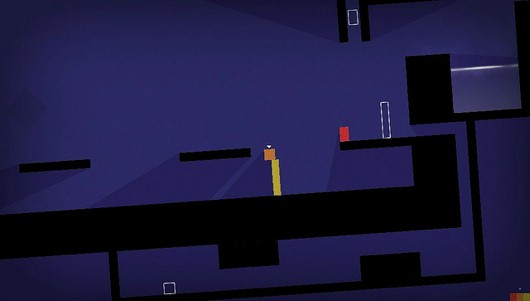
\includegraphics[width=7cm, height=5cm]{./figures/thomas.jpg}

Illumine contributed lighting and shading, and lots of it.  We initially did not know the direction we wanted to go in when designing the particle effects and lighting, and this
showed early on.  As we developed the game, however, we quickly realized we could leverage lighting to our advantage, and used it to hide all sorts of stuff from the player, such
as hidden passageways and enemy traps.  This lighting bled from the dungeon, where it originated, into the overworld, allowing some crazy overworld designs, such as writing words on the 
map and literally using it as an obstacle.  The player would never know the difference because they can't see all of it.

Here is an image from Illumine:

\includegraphics*[width=7cm, height=5cm]{./figures/illumine.png}

Finally, Legend of Zelda contributed the map style.  The map style of Legend of Zelda played very nicely with our lighting and shadow style, allowing for almost hidden feeling rooms,
dark dungeons, and otherwise visually interesting areas.  This primarily made its way into the overworld, with the dungeon being a more linear straight shot through, but traces 
of the Legend of Zelda dungeon style can still be seen in the dungeon layout.

Here is an image from Legend of Zelda:

\includegraphics*[width=7cm, height=5cm]{./figures/zelda.png}
\section{Changes from Initial Design}
We initially planned on this to be combat-centric, focusing on the spells and systems therein.  This changed drastically once we realized what was possible with our given inspirations, and we combined 
the three in a different way.  What began as a spell-caster morphed into an exploration game with combat on the side, with lighting growing to be the main focus.  The combat just wasn't anywhere near
as interesting as the lighting, nor was it as eye-popping as some of the visual effects we experimented with along the way.

Lighting played a huge role once we decided on shapes and colors.  Dim or bright lights began to take on meaning, while colors began denoting friend or foe.  
This was the point during which the game experienced the largest growing pain, that being the shift in focus from combat to lighting.  
This required the offshoot areas, part of the overworld, and the dungeon to go back to the drawing board for a bit.  While this did set us back a little, we were still able to deliver the project in 
a timely manner.

Once we had lighting figured out, shadows were a natural next step, and it did not disappoint.  The ability to combine creative shapes and colors with shadows to hide most of it created 
an environment the player wanted to explore, rather than an environment the player had already visually explored upon immediately entering any given room.  We tossed around the idea 
of having light be an environmental thing and the player casting these shadows, but this was quickly scrapped due to implementation difficulty and lack of interesting visual choice.

The puzzles were a massive paradigm shift from the original combat idea.  We went from being a game about combat, elemental interactions, and spell-slinging, to a focus on visual design, 
exploration, and detail.  This was, by far, both the biggest change in the project as well as the easiest.  We had a very easy time making the transition, even though it was sudden and required us to return 
to the drawing board for large chunks of the game.

Here is what our design looked like before the consideration; Dull and flat, with little room for improvement in the direction we were going.

\includegraphics*[width=7cm, height=5cm]{./figures/earlyproj.png}

Here is the game with updated lighting, which we considered a massive improvement upon what we were planning originally.

\includegraphics*[width=7cm, height=5cm]{./figures/ourgame.png}

Another leap in development occurred with particles, shortly after lighting.  Particles were something we wanted in some capacity, since they were usually good indicators and good player feedback, but 
we weren't sure how or where we wanted them.  Eventually we started with just basic door destruction particles, then went to plate activation particles, then on to damage particles.  This provided a 
sense of feedback for the player so they knew when they did something meaningful to the surrounding world.

A lesser discussed aspect that changed was a lot of back-end implementational details.  We fundamentally changed how the spells worked at least once or twice behind the scenes, and the 
spells were their own separate nightmare to get working.  Once we got spells working, though, not too much else got reworked side from one major code overhaul for the dungeon and its mechanics.

\section{Planning and Pre-Development}
Before we began development, we did plenty of tabletop planning.  This planning included hand-drawn and digital sketches of dungeon, overworlds, 
and offshoot areas, as well as enemy designs, boss designs, and player designs.  Some of the digital planning was done using Google sheets\cite{googlesheets} to "map" out the dungeon, overworld, and offshoot areas.

\includegraphics*[width=7cm, height=5cm]{./figures/designexample.png}

We also originally planned the spell system fairly extensively.  We discussed having four elements with a rock-paper-scissors style relation that also worked backwards for resistances.  This way, the player would always have at least one element they were super-effective against and two they were neutral against.  This, however, did not make it into the final product for change of focus from spellcasting to adventuring.

When planning the dungeon, we drew up several designs.  One design was a spider-web design, with the player entering in the center and branching out to fight several bosses.  Another design was a linear straight-line design, where the player simply battled down a hallway.  Another design was a maze-like array of rooms, which we ended up settling on, ending in a final boss room.

\includegraphics*[width=7cm, height=5cm]{./figures/DungeonLayout.png}

When planning the offshoot areas, almost all of them made it into the final product.  Only a couple were scrapped, which we are fairly proud of.  The offshoot areas were planned roughly the same way as the dungeon, mainly on Google sheets.

When planning the overworld, we planned it in chunks.  Rather than plan each room individually, we planned how the rooms would be laid out, then dropped the room designs in.  This proved to be quite effective for designing an interesting overworld.

\includegraphics*[width=7cm, height=5cm]{./figures/overworld.png}
We did spend an unusually large amount of time during this planning and pre-development stage, but it did not hurt the final product too bad in the long run.  We got nearly all the features implemented that we wanted, despite the time block dedicated to planning chewing up a lot of our time.

\section{Bumps We Hit Along the Way}
One bump we hit was lighting.  Even though it was a central focus of the game, it caused a fair amount of problems early on in implementation thanks to how godot handles lighting and shadows.  
In godot, lighting and shadows are handled based on lighting layers, which is not uncommon.  The strange bit, however, is the occlusion detection - it does not automatically occlude light 
when you define occlusion boundaries.
You must tell the light it is specifically allowed to cast a shadow, then define occlusion boundaries - this was not made abundantly clear in the 
documentation during creation of the lighting systems within the game, which set us back a tiny bit.  You also must use a CanvasModulate node, which applies a filter over the camera/viewport, 
to darken the scene so the shadows will actually show up and the light will have an effect.  This, also, was not made abundantly clear in the documentation when designing the lighting.  
These options are extremely flexible and allow for very fancy lights and shadows, but attempting to get them working was a minor hassle.

Another hurdle to get over was vector-based movement. Like said earlier, game developement was something we all were not very experienced in; And vector-based movement is vital to almost every
project that goes beyond a simple, non-stop side scroller. When this was initially approached, we wanted to implent this into our spellcasting for the projectile movement. With a little research
done for general game developement, the first attempt was making a Vector variable that was the product of a directional vector and any arbitrary speed value we chose and then just trying to apply
it directly to an instance of our projectile (or in other words, a projectile that we spawn as part of spellcasting). Once we played around with it and tried different things, we actually settled
on simply changing the \emph{local} y-coordinates every frame by a set amount, until the projectile collided with something or was far enough away. With that taken care of, we moved on to different
things, including enemies. Enemies were its own bag of fun, but ultimately we could not compromise on vector-based movement here. This took way longer than it should of, but eventually with the help
of the magic we call "team work", we were able to implement this. I will save the trouble of all the details, but we were fairly close to what our initial idea of how vector based movement should work.
Godot just has a particular way that it likes to handle this type of movement in a 2D space, and it was simply a matter of getting a better understanding of our tools available to us.

We had to learn to work with the tools we were given.  For some of us, that was easy to do.  For others, it was more difficult.  We are used to recreating all the tools we need from scratch, so learning to work within an engine was difficult for us at first.  We attempted to recreate our tools yet again, only to learn that they were built into the engine, and such was not necessary.

We also ran into problems with organizing our time and teamwork effectively.  Our teamwork was not really there; we operated as a group of individuals rather than a team and we frequently went off and worked on whatever aspect looked most interesting to us at the time.  This hindered possibilities for what could be developed moving forwards, and is something we would all change if given the chance.

We struggled with time management as well.  We spent an absorbent amount of time planning out our game, which chewed into our development time and forced some crunch time.  While we are not unfamiliar with crunch time, it happened too frequently for comfort, and is something we wish we could go back and change if given the opportunity.  


\section{Conclusion}
\emph{Project Spellda} came out well overall, especially considering the time frame and experience that we had. The game was designed with the lighting style in mind, and uses this lighting style
to give a better over-all feel to the games appearance and gameplay. There is a working tutorial level with working pickups and enemies. There is an overworld to explore with enemies and other pathways
to offshoot areas with their own challenges and looks. There is a dungeon with puzzles and enemies, with a boss to finish out the gameplay. We accomplished all of this using Godot and the native
language, GDScript. All three group members learned a great deal from this, and plan to take what they learned throughout the project with their own, individual projects as hobbies.


\bibliographystyle{plain}
\bibliography{bibliography}

\end{document}
